\chapter{Results} % Main chapter title

\label{Chapter7} % For referencing this chapter elsewhere, use \ref{Chapter7}

\lhead{Chapter 7. \emph{Results}}

%----------------------------------------------------------------------------------------
%	SECTION 7.1 - Results
%----------------------------------------------------------------------------------------

\section{Results}

%----------------------------------------------------------------------------------------
%	SUBSECTION 7.1.1 - Results Graphs
%----------------------------------------------------------------------------------------

\subsection{Results Graphs}

This section will present several graphs taken from data extracted throughout the experiments. First of all, precisions are needed on the experiments themselves. \emph{Brevitas} is still in development and several functionalities are still missing. While the main idea was to use several well-known network architectures (\emph{LeNet-5}, \emph{AlexNet}, \emph{VGG}, and \emph{Mobilenet}), the reality is that most of these networks are not yet supported by the export functionality. This export is crucial as it allows one to port its \emph{Brevitas}-defined and trained network and export it to \emph{ONNX} before importing it in \emph{FINN} and deploying it on an FPGA.

In the end, out of the three networks presented in the last chapter, only the \emph{TFC} network can make the full run, through training, export and on FPGA. The \emph{CNV} network gets stuck through several transformations and sequence of layers that are not yet supported by the streamlining process. On the other hand, \emph{MobilenetV1} is not even exporting to \emph{ONNX} and was chosen to be stopped.

However, \emph{TFC} training results can be seen on \emph{Figure} \ref{fig:TFCErrorRate} where the different configuration A\emph{X}W\emph{X}, where \emph{X} is the bit-width of both activations and weights. The different configurations have been trained for 40 epochs in total and a model has been kept for evaluation every 10 epochs. The graph represents the error rate (or $100 - accuracy$) given the training time.

% GRAPH ACCURACY TRAINING TIME TFC
\begin{figure}[htbp]
\centering
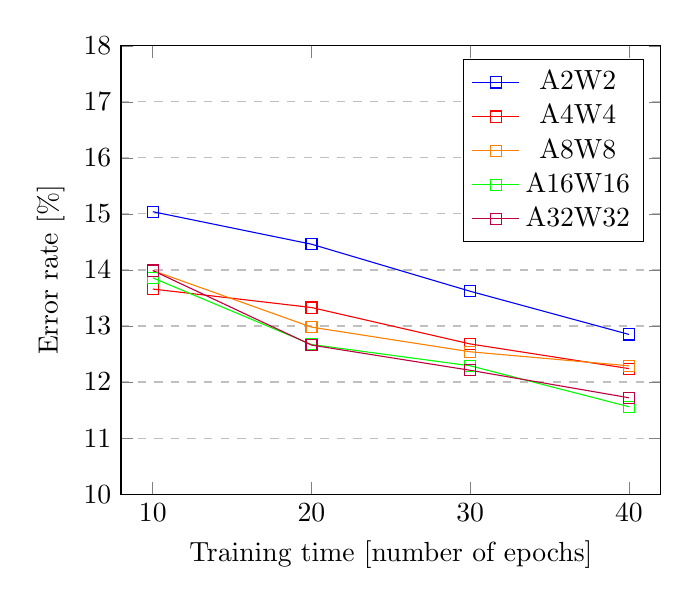
\begin{tikzpicture}
\begin{axis}[
    xlabel={Training time [number of epochs]},
    ylabel={Error rate [\%]},
    xmin=8, xmax=42,
    ymin=10, ymax=18,
    xtick={0,10,20,30,40},
    ytick={10,11,12,13,14,15,16,17,18},
    legend pos=north east,
    ymajorgrids=true,
    grid style=dashed,
]
% TFC A2W2:   84.960 | 85.540 | 86.380 | 87.150
\addplot[
    color=blue,
    mark=square,
    ]
    coordinates {
    (10,15.04)(20,14.46)(30,13.62)(40,12.85)
    };
% TFC A4W4:   86.340 | 86.670 | 87.320 | 87.760
\addplot[
    color=red,
    mark=square,
    ]
    coordinates {
    (10,13.66)(20,13.33)(30,12.68)(40,12.24)
    };
% TFC A8W8:   86.010 | 87.020 | 87.460 | 87.710
\addplot[
    color=orange,
    mark=square,
    ]
    coordinates {
    (10,13.99)(20,12.98)(30,12.54)(40,12.29)
    };
% TFC A16W16: 86.140 | 87.330 | 87.710 | 88.440
\addplot[
    color=green,
    mark=square,
    ]
    coordinates {
    (10,13.86)(20,12.67)(30,12.29)(40,11.56)
    };
% TFC A32W32: 86.010 | 87.340 | 87.690 | 88.280
\addplot[
    color=purple,
    mark=square,
    ]
    coordinates {
    (10,13.99)(20,12.66)(30,12.21)(40,11.72)
    };
\legend{A2W2,A4W4,A8W8,A16W16,A32W32}
\end{axis}
\end{tikzpicture}
\caption[TFC Error Rate]{TFC error rate against training time}
  \label{fig:TFCErrorRate}
\end{figure}

While the \emph{CNV} network could not be deployed, it could still be trained and the results can be seen on \emph{Figure} \ref{fig:CNVErrorRate}. As in the \emph{TFdC} figure, the configurations are named A\emph{X}W\emph{X}, where \emph{X} is the bit-width.

% GRAPH ACCURACY TRAINING TIME CNV
\begin{figure}[htbp]
\centering
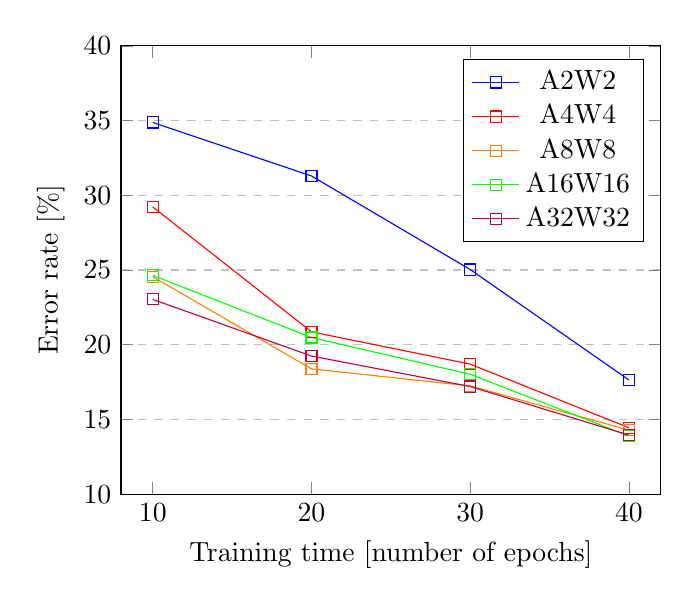
\begin{tikzpicture}
\begin{axis}[
    xlabel={Training time [number of epochs]},
    ylabel={Error rate [\%]},
    xmin=8, xmax=42,
    ymin=10, ymax=40,
    xtick={0,10,20,30,40},
    ytick={10,15,20,25,30,35,40},
    legend pos=north east,
    ymajorgrids=true,
    grid style=dashed,
]
% CNV A2W2:   65.130 | 68.710 | 76.970 | 82.360
\addplot[
    color=blue,
    mark=square,
    ]
    coordinates {
    (10,34.87)(20,31.29)(30,25.03)(40,17.64)
    };
% CNV A4W4:   70.780 | 79.140 | 81.300 | 85.560
\addplot[
    color=red,
    mark=square,
    ]
    coordinates {
    (10,29.22)(20,20.86)(30,18.70)(40,14.44)
    };
% CNV A8W8: 75.450 | 81.620 | 82.760 | 85.720
\addplot[
    color=orange,
    mark=square,
    ]
    coordinates {
    (10,24.55)(20,18.38)(30,17.24)(40,14.28)
    };
% CNV A16W16: 75.360 | 79.520 | 81.980 | 86.110
\addplot[
    color=green,
    mark=square,
    ]
    coordinates {
    (10,24.64)(20,20.48)(30,18.02)(40,13.89)
    };
% CNV A32W32: 72.970 | 80.760 | 82.800 | 86.050
\addplot[
    color=purple,
    mark=square,
    ]
    coordinates {
    (10,23.03)(20,19.24)(30,17.20)(40,13.95)
    };

\legend{A2W2,A4W4,A8W8,A16W16,A32W32}
\end{axis}
\end{tikzpicture}
\caption[CNV Error Rate]{CNV error rate against training time}
  \label{fig:CNVErrorRate}
\end{figure}

The \emph{TFC} graph (\emph{Figure} \ref{TFCErrorRate}) shows a separation in three sections: 2-bits precision, 4- and 8-bits precision and 16- and 32-bits precision. This separation is seen in terms of reaction to the training. The result of the training, after 40 epochs shows three separate points: $\sim$13\% error rate for A2W2, $\sim$12.3\% error rate for A4W4 and A8W8 and $\sim$11.6\% for A16E16 and A32W32. On the other hand for the \emph{CNV} network, there is a clear separation between A2W2 at $\sim$17.5\% and all the other configurations at $\sim$14.8\%.

Now if we look deeper into the \emph{TFC} deployment, we can get other important metrics from the experiments. First, \emph{Figure} \ref{fig:TFCThroughput} shows the throughput compared to the error rate determined earlier. Note that the error rate for a 40-epochs long training is used.

The three metrics presented in the next graphs are: \emph{throughput}, the number of images the deployed network can process in one second ; \emph{DRAM in bandwidth}, the amount of data that can be processed coming from the DRAM in to the FPGA board ; \emph{DRAM out banwidth}, the amount of data that can be processed coming from the FPGA board out to the DRAM.

\begin{itemize}
  \item \textbf{Throughput}(\emph{Figure} \ref{fig:TFCThroughput}): If the throughput seems nearly identical for A2W2 and A4W4, going to A8W8 makes one lose more than 10 thousands images per second. And even worse, using A16W16 consists of a loss of over 45 thousands images per second.

  % THROUGHPUT FIGURE
  \begin{figure}[htbp]
  \centering
  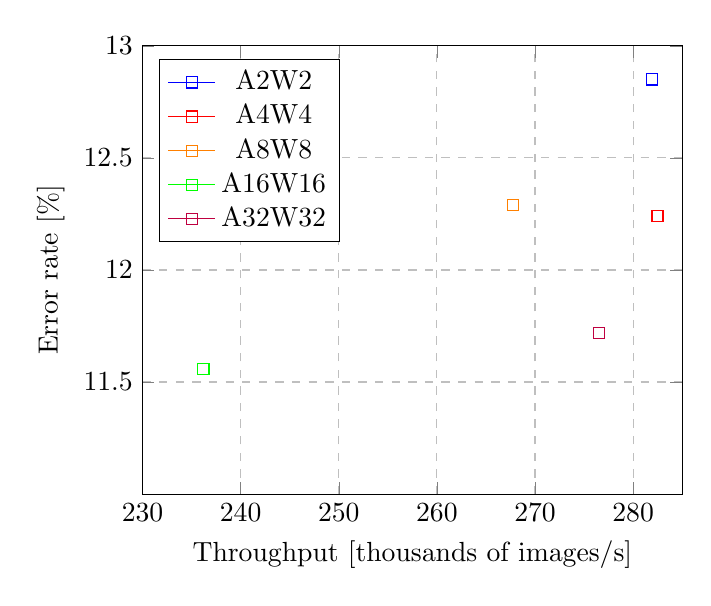
\begin{tikzpicture}
  \begin{axis}[
    xlabel={Throughput [thousands of images/s]},
    ylabel={Error rate [\%]},
    xmin=230, xmax=285,
    ymin=11, ymax=13,
    xtick={230,240,250,260,270,280},
    ytick={11.5,12,12.5,13},
    legend pos=north west,
    ymajorgrids=true,
    xmajorgrids=true,
    grid style=dashed,
    ]
  % A2W2
  \addplot+ [
      color=blue,
      mark=square
      ] coordinates {(281.951,12.85)};
  % A4W4
  \addplot+ [
      color=red,
      mark=square
      ] coordinates {(282.483,12.24)};
  % A8W8
  \addplot+ [
      color=orange,
      mark=square
      ] coordinates {(267.732,12.29)};
  % A16W16
  \addplot+ [
      color=green,
      mark=square
      ] coordinates {(236.205,11.56)};
  % A32W32
  \addplot+ [
      color=purple,
      mark=square
      ] coordinates {(276.541,11.72)};
  \legend{A2W2,A4W4,A8W8,A16W16,A32W32}
  \end{axis}
  \end{tikzpicture}
  \caption[TFC Throughput]{TFC error rate compared to throughput}
    \label{fig:TFCThroughput}
  \end{figure}


  \item \textbf{DRAM in bandwidth}(\emph{Figure} \ref{fig:TFCDRAMIn}): The same conclusions can be used for the DRAM bandwidth. The more the bit-width, the lower the bandwidth, with an exception fo A4W4 that outperforms A2W2 being at 288 against 283 Mb/s.

  % DRAM in bandwidth FIGURE
  \begin{figure}[htbp]
  \centering
  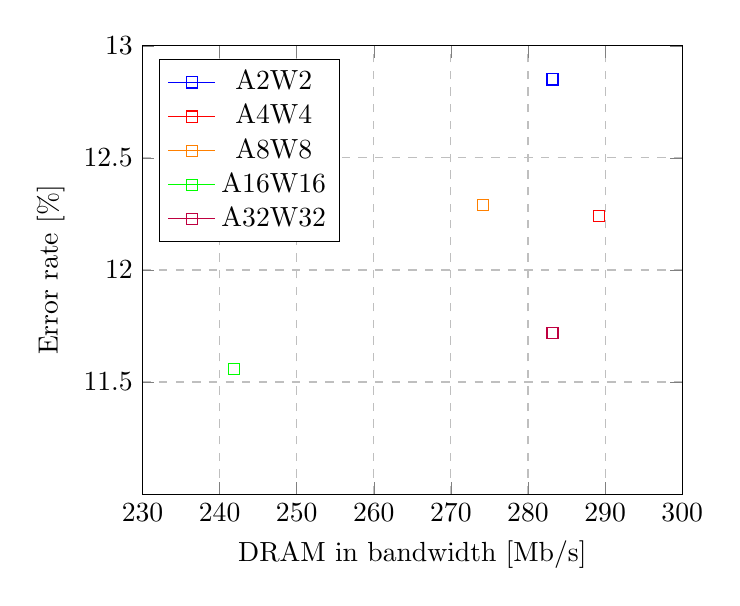
\begin{tikzpicture}
  \begin{axis}[
    xlabel={DRAM in bandwidth [Mb/s]},
    ylabel={Error rate [\%]},
    xmin=230, xmax=300,
    ymin=11, ymax=13,
    xtick={230,240,250,260,270,280,290,300},
    ytick={11.5,12,12.5,13},
    legend pos=north west,
    ymajorgrids=true,
    xmajorgrids=true,
    grid style=dashed,
    ]
  % A2W2
  \addplot+ [
      color=blue,
      mark=square
      ] coordinates {(283.18,12.85)};
  % A4W4
  \addplot+ [
      color=red,
      mark=square
      ] coordinates {(289.26,12.24)};
  % A8W8
  \addplot+ [
      color=orange,
      mark=square
      ] coordinates {(274.16,12.29)};
  % A16W16
  \addplot+ [
      color=green,
      mark=square
      ] coordinates {(241.87,11.56)};
  % A32W32
  \addplot+ [
      color=purple,
      mark=square
      ] coordinates {(283.18,11.72)};
  \legend{A2W2,A4W4,A8W8,A16W16,A32W32}
  \end{axis}
  \end{tikzpicture}
  \caption[TFC DRAM in]{TFC DRAM in bandwidth when compared to error rate}
    \label{fig:TFCDRAMIn}
  \end{figure}

  \item \textbf{DRAM out bandwidth}(\emph{Figure} \ref{fig:TFCDRAMOut}): While the graph presents the same impressions as the DRAM in, the results for A2W2 and A4W4 are this time nearly identical around 11.3Mb/s


  % DRAM out bandwidth FIGURE
  \begin{figure}[htbp]
  \centering
  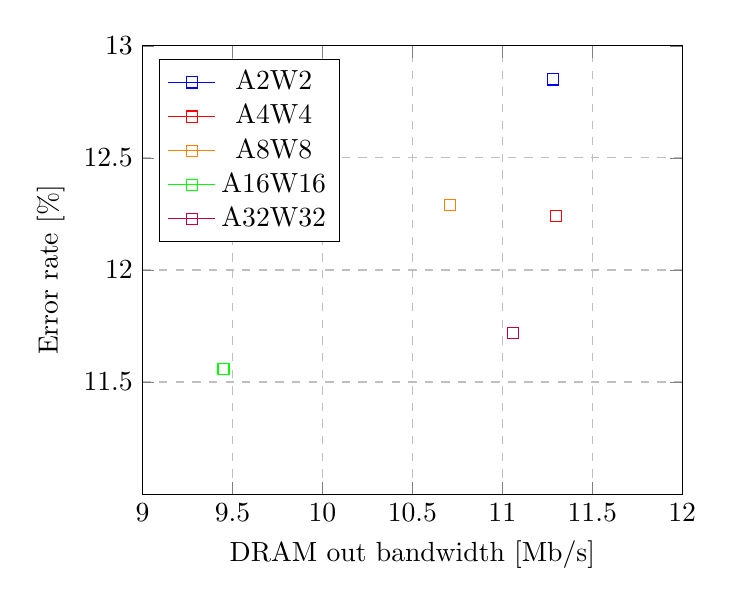
\begin{tikzpicture}
  \begin{axis}[
    xlabel={DRAM out bandwidth [Mb/s]},
    ylabel={Error rate [\%]},
    xmin=9, xmax=12,
    ymin=11, ymax=13,
    xtick={9,9.5,10,10.5,11,11.5,12},
    ytick={11.5,12,12.5,13},
    legend pos=north west,
    ymajorgrids=true,
    xmajorgrids=true,
    grid style=dashed,
    ]
  % A2W2
  \addplot+ [
      color=blue,
      mark=square
      ] coordinates {(11.28,12.85)};
  % A4W4
  \addplot+ [
      color=red,
      mark=square
      ] coordinates {(11.30,12.24)};
  % A8W8
  \addplot+ [
      color=orange,
      mark=square
      ] coordinates {(10.71,12.29)};
  % A16W16
  \addplot+ [
      color=green,
      mark=square
      ] coordinates {(9.45,11.56)};
  % A32W32
  \addplot+ [
      color=purple,
      mark=square
      ] coordinates {(11.06,11.72)};
  \legend{A2W2,A4W4,A8W8,A16W16,A32W32}
  \end{axis}
  \end{tikzpicture}
  \caption[TFC DRAM out]{TFC DRAM out bandwidth when compared to error rate}
    \label{fig:TFCDRAMOut}
  \end{figure}
\end{itemize}


%----------------------------------------------------------------------------------------
%	SUBSECTION 7.1.2 - Results Tables
%----------------------------------------------------------------------------------------
\newpage
\subsection{Results Tables}

This section presents the data used to plot the different graphs from earlier as well as other metrics that have been gathered from the Vivado implementation. The first two tables, \emph{Table} \ref{tab:TFCAccuracyTable} and \emph{Table} \ref{tab:CNVAccuracyTable}, present the accuracy obtained when training \emph{TFC} and \emph{CNV} for 40 epochs, using a checkpoint every 10 epochs.

\begin{table}[!htb]
  \centering
  \resizebox{\textwidth}{!}{
  \begin{tabular}{ | c | c | c | c | c | }
    \hline
    \textbf{Experiment Name} & \textbf{10 epochs} & \textbf{20 epochs} & \textbf{30 epochs} & \textbf{40 epochs} \\
    \hline
    \textbf{A2W2}          & 84.960 & 85.540 & 86.380 & 87.150 \\
    \hline
    \textbf{A4W4}          & 86.340 & 86.670 & 87.320 & 87.760 \\
    \hline
    \textbf{A8W8}          & 86.010 & 87.020 & 87.460 & 87.710 \\
    \hline
    \textbf{A16W16}       & 86.140 & 87.330 & 87.710 & 88.440 \\
    \hline
    \textbf{A32W32}       & 86.010 & 87.340 & 87.690 & 88.280 \\
    \hline
  \end{tabular}
  }
\caption[TFC Accuracy Table]{TFC accuracy for different training times}
\label{tab:TFCAccuracyTable}
\end{table}

% Results for Accuracy 10 | 20 | 30 | 40 epochs
% A2W2:   84.960 | 85.540 | 86.380 | 87.150
% A4W4:   86.340 | 86.670 | 87.320 | 87.760
% A8W8:   86.010 | 87.020 | 87.460 | 87.710
% A16W16: 86.140 | 87.330 | 87.710 | 88.440
% A32W32: 86.010 | 87.340 | 87.690 | 88.280

For the \emph{TFC} example in \emph{Table} \ref{tab:TFCAccuracyTable}, there is a difference in accuracy of 1.13\% between the 2-bits and 32-bits after 40 epochs of training. Moreover, there is only a difference of 0.9\% between the 2-bits version after 40 epochs and the 32-bits version after 20 epochs. While lower bits representations need more time to train, they can achieve similar result to a certain extent.

\begin{table}[!htb]
  \centering
  \resizebox{\textwidth}{!}{
  \begin{tabular}{ | c | c | c | c | c | }
    \hline
    \textbf{Experiment Name} & \textbf{10 epochs} & \textbf{20 epochs} & \textbf{30 epochs} & \textbf{40 epochs} \\
    \hline
    \textbf{A2W2I8}          & 65.130 & 68.710 & 76.970 & 82.360 \\
    \hline
    \textbf{A4W4I8}          & 70.780 & 79.140 & 81.300 & 85.560 \\
    \hline
    \textbf{A8W8I8}          & 75.450 & 81.620 & 82.760 & 85.720 \\
    \hline
    \textbf{A16W16I32}       & 75.360 & 79.520 & 81.980 & 86.110 \\
    \hline
    \textbf{A32W32I32}       & 72.970 & 80.760 & 82.800 & 86.050 \\
    \hline
  \end{tabular}
  }
\caption[CNV Accuracy Table]{CNV accuracy for different training times}
\label{tab:CNVAccuracyTable}
\end{table}

% Results for Accuracy 10 | 20 | 30 | 40 epochs
% A2W2:   65.130 | 68.710 | 76.970 | 82.360
% A4W4:   70.780 | 79.140 | 81.300 | 85.560
% A8W8:   75.450 | 81.620 | 82.760 | 85.720
% A16W16: 75.360 | 79.520 | 81.980 | 86.110
% A32W32: 72.970 | 80.760 | 82.800 | 86.050

The \emph{CNV} case in \emph{Table} \ref{tab:CNVAccuracyTable} presents the same conclusions. While there is a difference of 7.84\% between the 2-bits and 32-bits accuracy after 10 epochs of training, this difference lowers to 4.3\% after 40 epochs for both. Moreover, if we compare the 2-bits accuracy after 40 epochs and the 32-bits accuracy after 30 epochs, there is on 0.44\% of difference in accuracy.

\begin{table}[!htb]
  \centering
  \resizebox{\textwidth}{!}{
  \begin{tabular}{ | c | c | c | c | c | }
    \hline
    \textbf{Experiment Name} & \textbf{Throughput} & \textbf{DRAM in bandwidth} & \textbf{DRAM out bandwidth} \\
    \hline
    \textbf{A2W2}          & 281951 [img/s]  & 283.18 [Mb/s] & 11.28 [Mb/s] \\
    \hline
    \textbf{A4W4}          & 282483 [img/s]  & 289.26 [Mb/s] & 11.30 [Mb/s] \\
    \hline
    \textbf{A8W8}          & 267732 [img/s]  & 274.16 [Mb/s] & 10.71 [Mb/s] \\
    \hline
    \textbf{A16W16}       & 236205 [img/s]  & 241.87 [Mb/s] &  9.45 [Mb/s] \\
    \hline
    \textbf{A32W32}       & 276541 [img/s]  & 283.18 [Mb/s] & 11.06 [Mb/s] \\
    \hline
  \end{tabular}
  }
\caption[TFC IO Table]{TFC I/O metrics}
  \label{tab:TFCIOTable}
\end{table}

% Results for            Throughput | DRAM in bandwidth | DRAM out bandwidth:
% A2W2:   281951 (img/s) | 283.18 (Mb/s)     | 11.28  (Mb/s)
% A4W4:   282483 (img/s) | 289.26 (Mb/s)     | 11.30  (Mb/s)
% A8W8:   267732 (img/s) | 274.16 (Mb/s)     | 10.71  (Mb/s)
% A16W16: 236205 (img/s) | 241.87 (Mb/s)     | 9.45   (Mb/s)
% A32W32: 276541 (img/s) | 283.18 (Mb/s)     | 11.06  (MB/s)

The other metrics include several I/O mechanics when looking at the DRAM in/out bandwidth and the underlying throughput. Those three metrics are presented in \emph{Table} \ref{tab:TFCIOTable}. From this table, we can see that, with an exception to A32W32, the lower the bit-width the higher the throughput and DRAM i/o bandwidth. However, A32W32 is coming third on the throughput test, DRAM in bandwidth and fourth on the DRAM out bandwidth.

\begin{table}[!htb]
  \centering
  \resizebox{\textwidth}{!}{
  \begin{tabular}{ | c | c | c | c | c | }
    \hline
    \textbf{Experiment Name} & \textbf{Power} & \textbf{Look-Up Tables} & \textbf{Flip-Flops} & \textbf{BRAM} \\
    \hline
    \textbf{A2W2}          & 2.140 [W]  & 30618 [57.55\%] & 27704 [26.04\%] &  41.5 [29.6\%] \\
    \hline
    \textbf{A4W4}          & 2.151 [W]  & 30644 [57.60\%] & 27760 [26.09\%] &  41.5 [29.6\%] \\
    \hline
    \textbf{A8W8}          & 2.070 [W]  & 30617 [57.55\%] & 27660 [26.09\%] &  41.5 [29.6\%] \\
    \hline
    \textbf{A16W16}        & 2.136 [W]  & 30610 [57.54\%] & 27717 [26.05\%] &  41.5 [29.6\%] \\
    \hline
    \textbf{A32W32}        & 2.159 [W]  & 30586 [57.49\%] & 27670 [26.01\%] &  41.5 [29.6\%] \\
    \hline
  \end{tabular}
  }
\caption[TFC Hardware Utilisation Table]{TFC Hardware Utilisation}
\label{tab:TFCHardwareTable}
\end{table}

Finally, hardware resources are available in \emph{Table} \ref{tab:TFCHardwareTable}. They present both the power needed to run the bitfile, the number of \emph{Look-Up Tables (LUT)} needed to synthesise the design, the number of \emph{Flip-Flops (FF)} as well as the \emph{BRAM Usage}. In terms of power, A8W8 consumes the less with 2.07W and S2W2 as well as A4W4 consume more (2.14W and 2.151 respectively) than A16W16 at 2.136W. A32W32 is well on top with 2.159W consumed. In terms of \emph{LUTs} and \emph{FFs}, A32W32 is the representation using the less \emph{LUTs} while A8W8 is the representation using the less \emph{FFs}. On the other hand, A4W4 uses the most \emph{LUTs} and \emph{FFs}. The \emph{BRAM} usage is the exact same for all the different representations. More information and more detailed hardware utilisation metrics can be seen in the \emph{Appendix A} \ref{AppendixA}.

%----------------------------------------------------------------------------------------
%	SUBSECTION 7.1.3 - Results Conclusion
%----------------------------------------------------------------------------------------

\subsection{Results Conclusion}

These results show several interesting insights on the representations. First of all, those results confirm that the workflow of \emph{Benchmark}, \emph{Brevitas}, \emph{ONNX}, \emph{FINN} is working and can allow one to port its neural networks on an FPGA board. The results on accuracy correspond to the intuition one might have on the idea of \guille{the higher the bit-width of weights and activations, the higher the overall accuracy of the network}. However, it highlights a small difference in accuracy between 2-bits and 32-bits representations, and even a more negligible difference between 32-bits and 40bits or 8-bits representations.

An unsettling result is the performance of the 32-bits representation in terms of I/O metrics. This representation outperforms several other contenders in terms of throughput and DRAM i/o bandwidth. This is while the 16-bit representation arrives last with an important difference in both throughput (40 thousands images when compared to the 2-bits representation) or DRAM bandwidth (40 Mb/s for the in bandwidth and 2 Mb/s for the out bandwidth).

Following the same way, hardware utilisation metrics show a similar usage of \emph{LUTs} between the representations, the 32-bits representation being the one using the less of them and nearly being the one using the less of \emph{FFs}. This is counter-intuitive as one would expect the \guille{biggest} representation to use the most hardware resources. However, the power consumption is the highest when dealing with this 32-bits representation.
